\documentclass[tikz,border=2mm]{standalone}
\usepackage{tikz}

\definecolor{red}{rgb}{1,.5,.6}
\definecolor{blue}{rgb}{.5,.5,1}

\begin{document}
	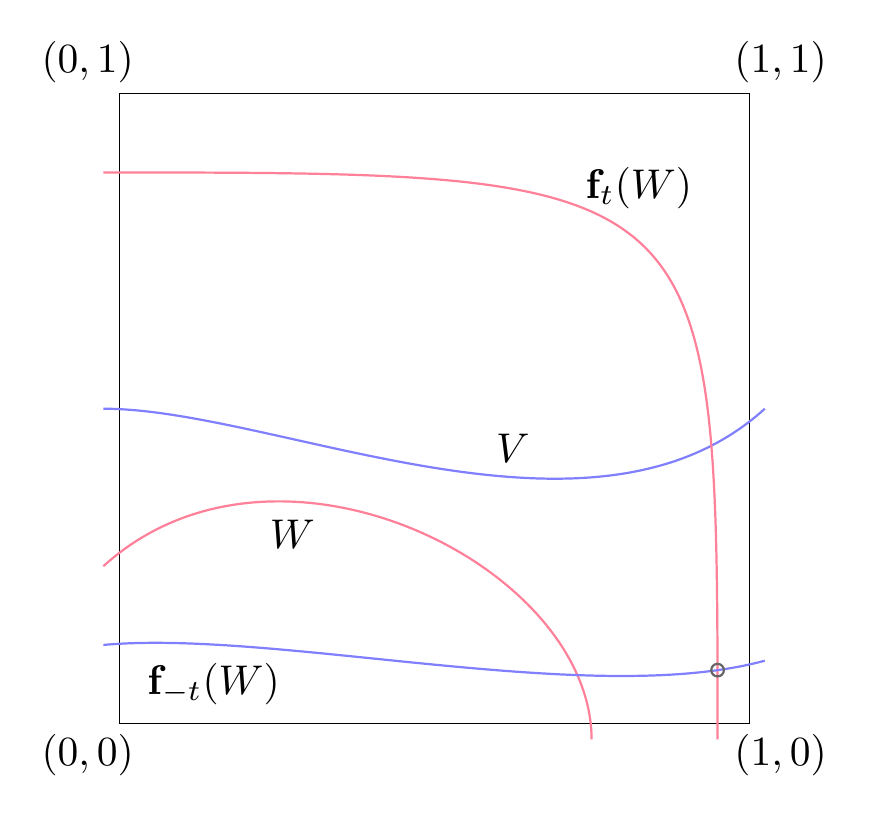
\begin{tikzpicture}[scale = 2]

	\draw (0,0) -- (0,4) -- (4,4) -- (4,0) -- (0,0);

	\draw[red, thick] (-.1,1) .. controls (1,2) and (3,1).. (3,-.1);
	\draw[blue, thick] (-.1,2) .. controls (1,2) and (3,1).. (4.1,2);
	\draw[red, thick] (-.1,3.5) .. controls (3.8,3.5) .. (3.8,-.1);
	\draw[blue, thick] (-.1,.5) .. controls (1,.6) and (3,.1).. (4.1,.4);

	\node[scale=1.5] at (-.2, -.2) {$(0,0)$};
	\node[scale=1.5] at (4.2, -.2) {$(1,0)$};
	\node[scale=1.5] at (4.2, 4.2) {$(1,1)$};
	\node[scale=1.5] at (-.2, 4.2) {$(0,1)$};

	\node[scale=1.5] at (1.1, 1.2) {$W$};
	\node[scale=1.5] at (2.5, 1.75) {$V$};
	\node[scale=1.5] at (3.3, 3.4) {$\mathbf f_t(W)$};
	\node[scale=1.5] at (.6, .25) {$\mathbf f_{-t}(W)$};

	\draw[color=black!60, thick](3.8,.34) circle (.04);
	\draw[circle,fill,radius=1000pt,black] (4,2);
	\end{tikzpicture}
\end{document}